GFE $\theta$ estimates are root-N consistent.

\begin{figure}[h]
\begin{flushleft}
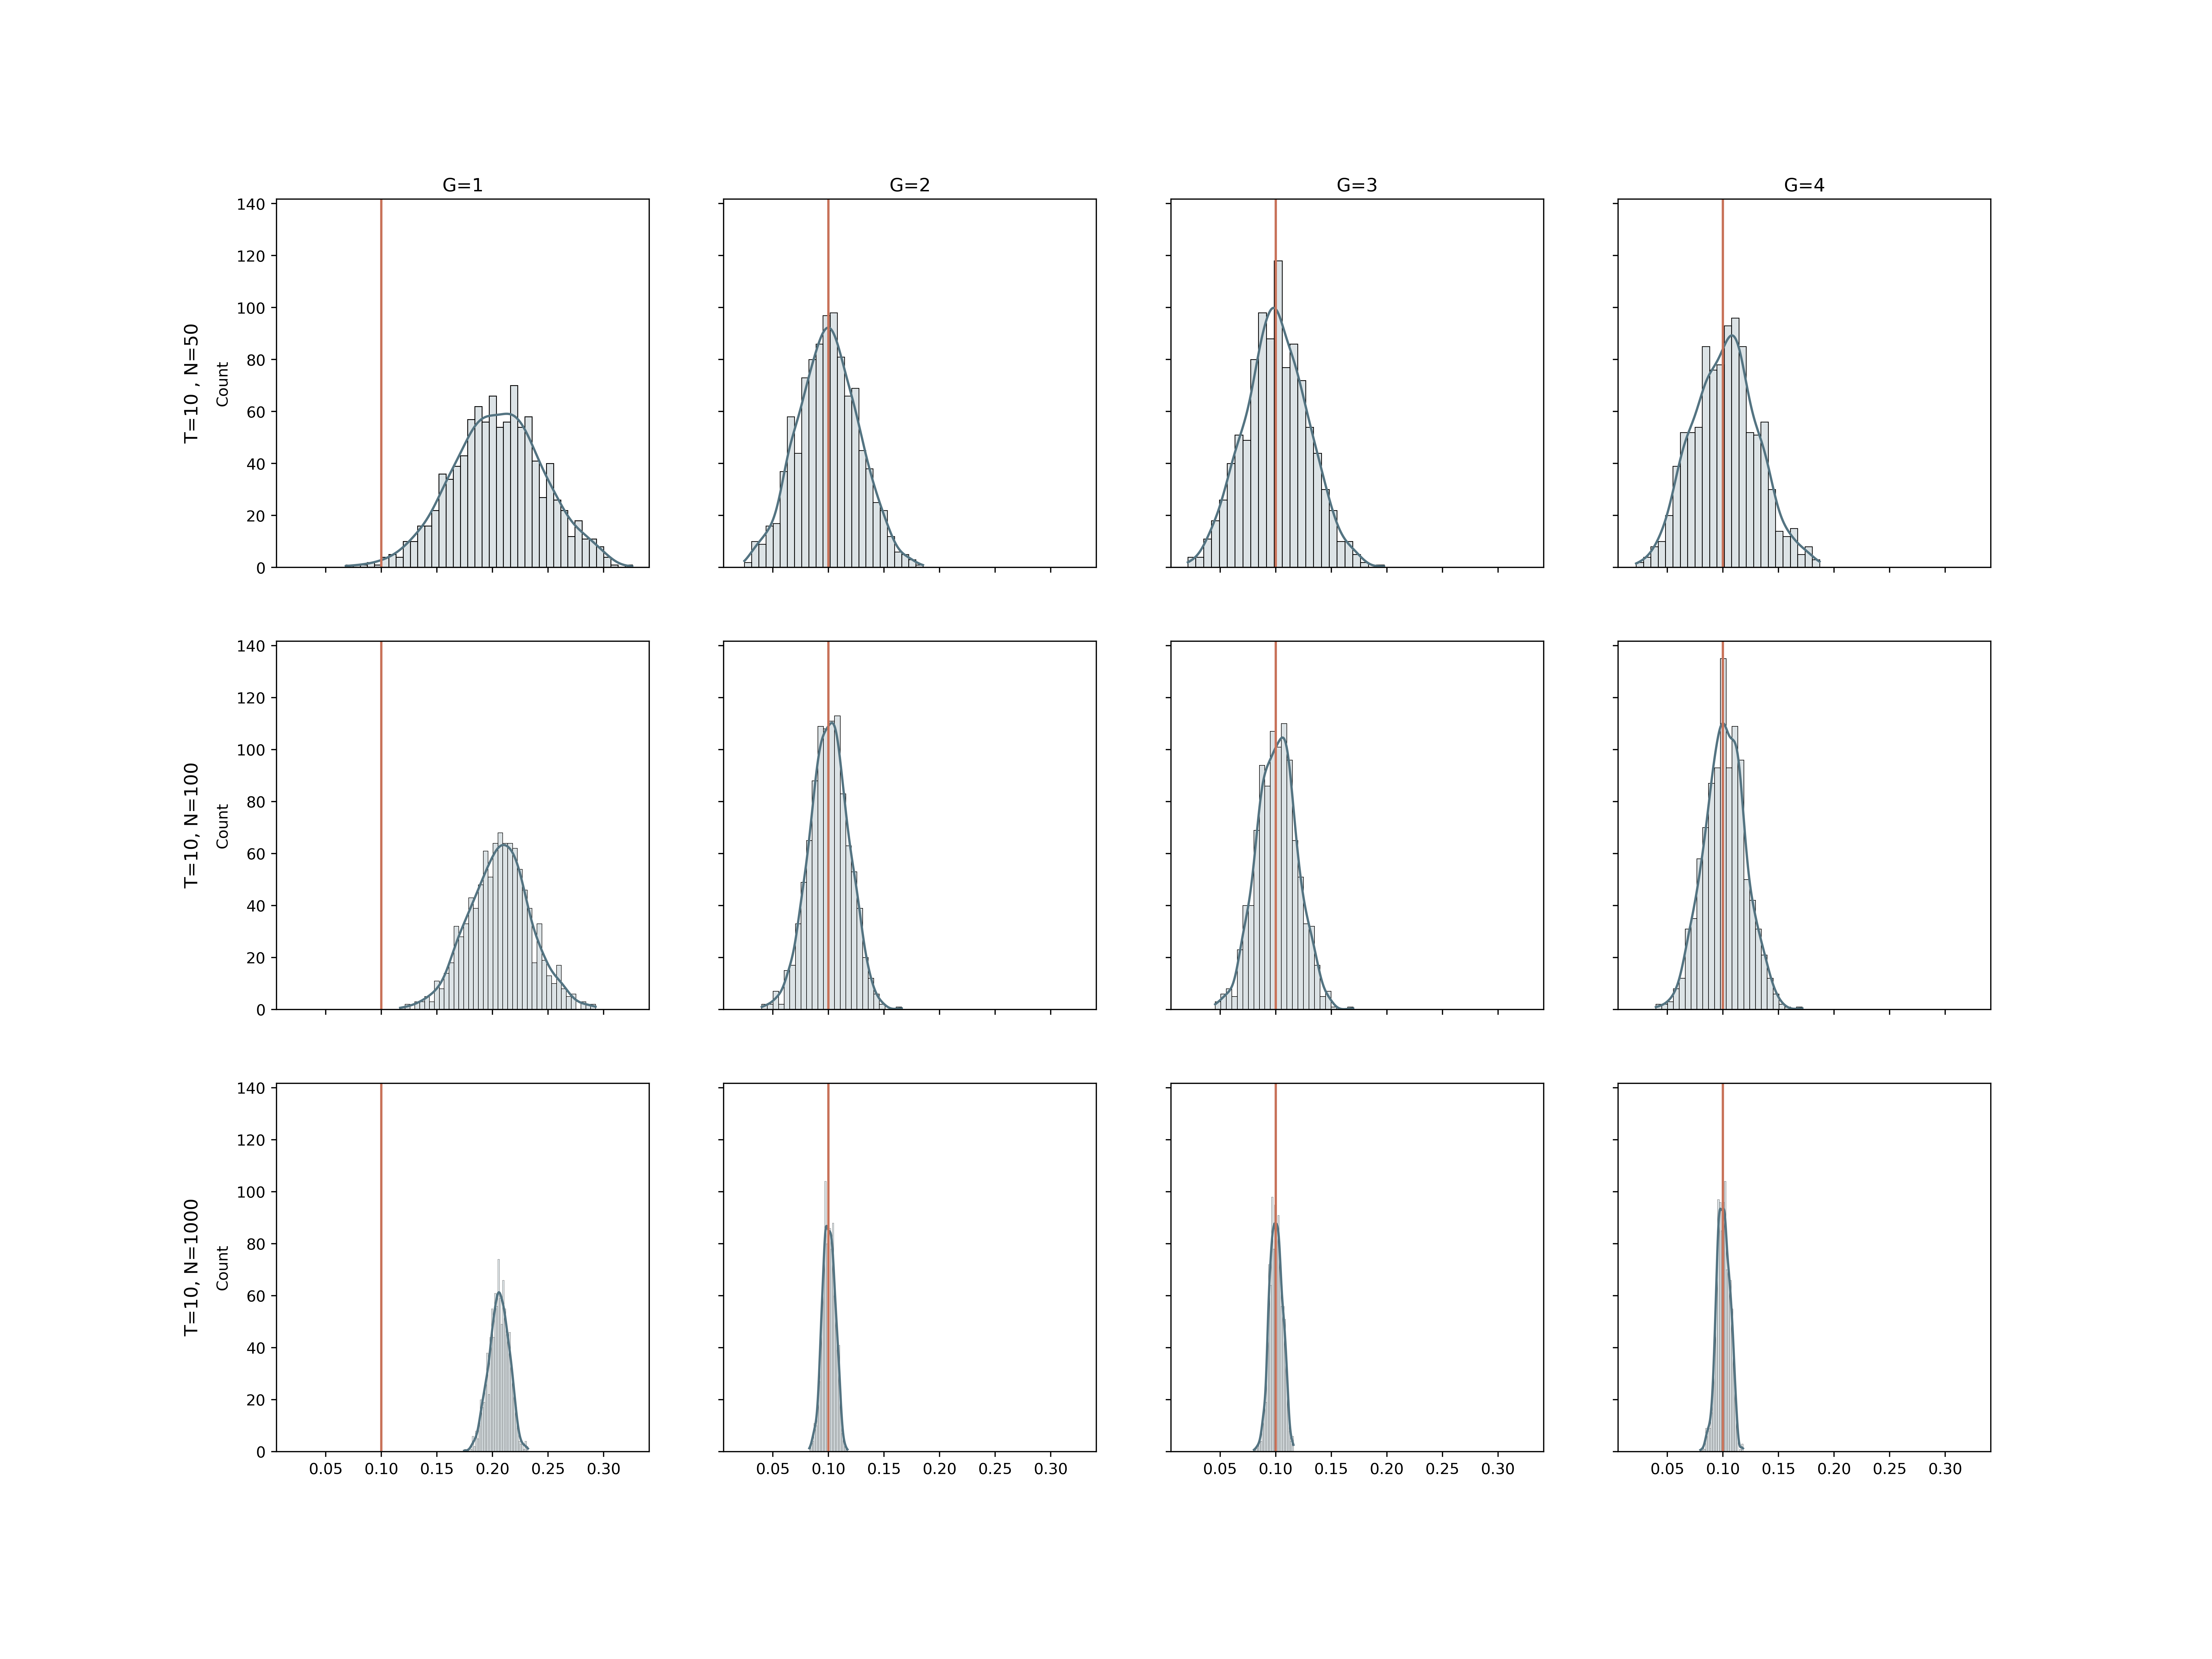
\includegraphics[scale=0.31]{sections/appendix/groupssamplingplotN1.png}
\end{flushleft}
\caption{Sampling Distribution of $\hat{\theta_1}$ when T=10 and N increases in different number of group specifications where $G^0 = 2$.}
\label{fig:gsn}
\end{figure}

\begin{figure}[h]
\begin{flushleft}
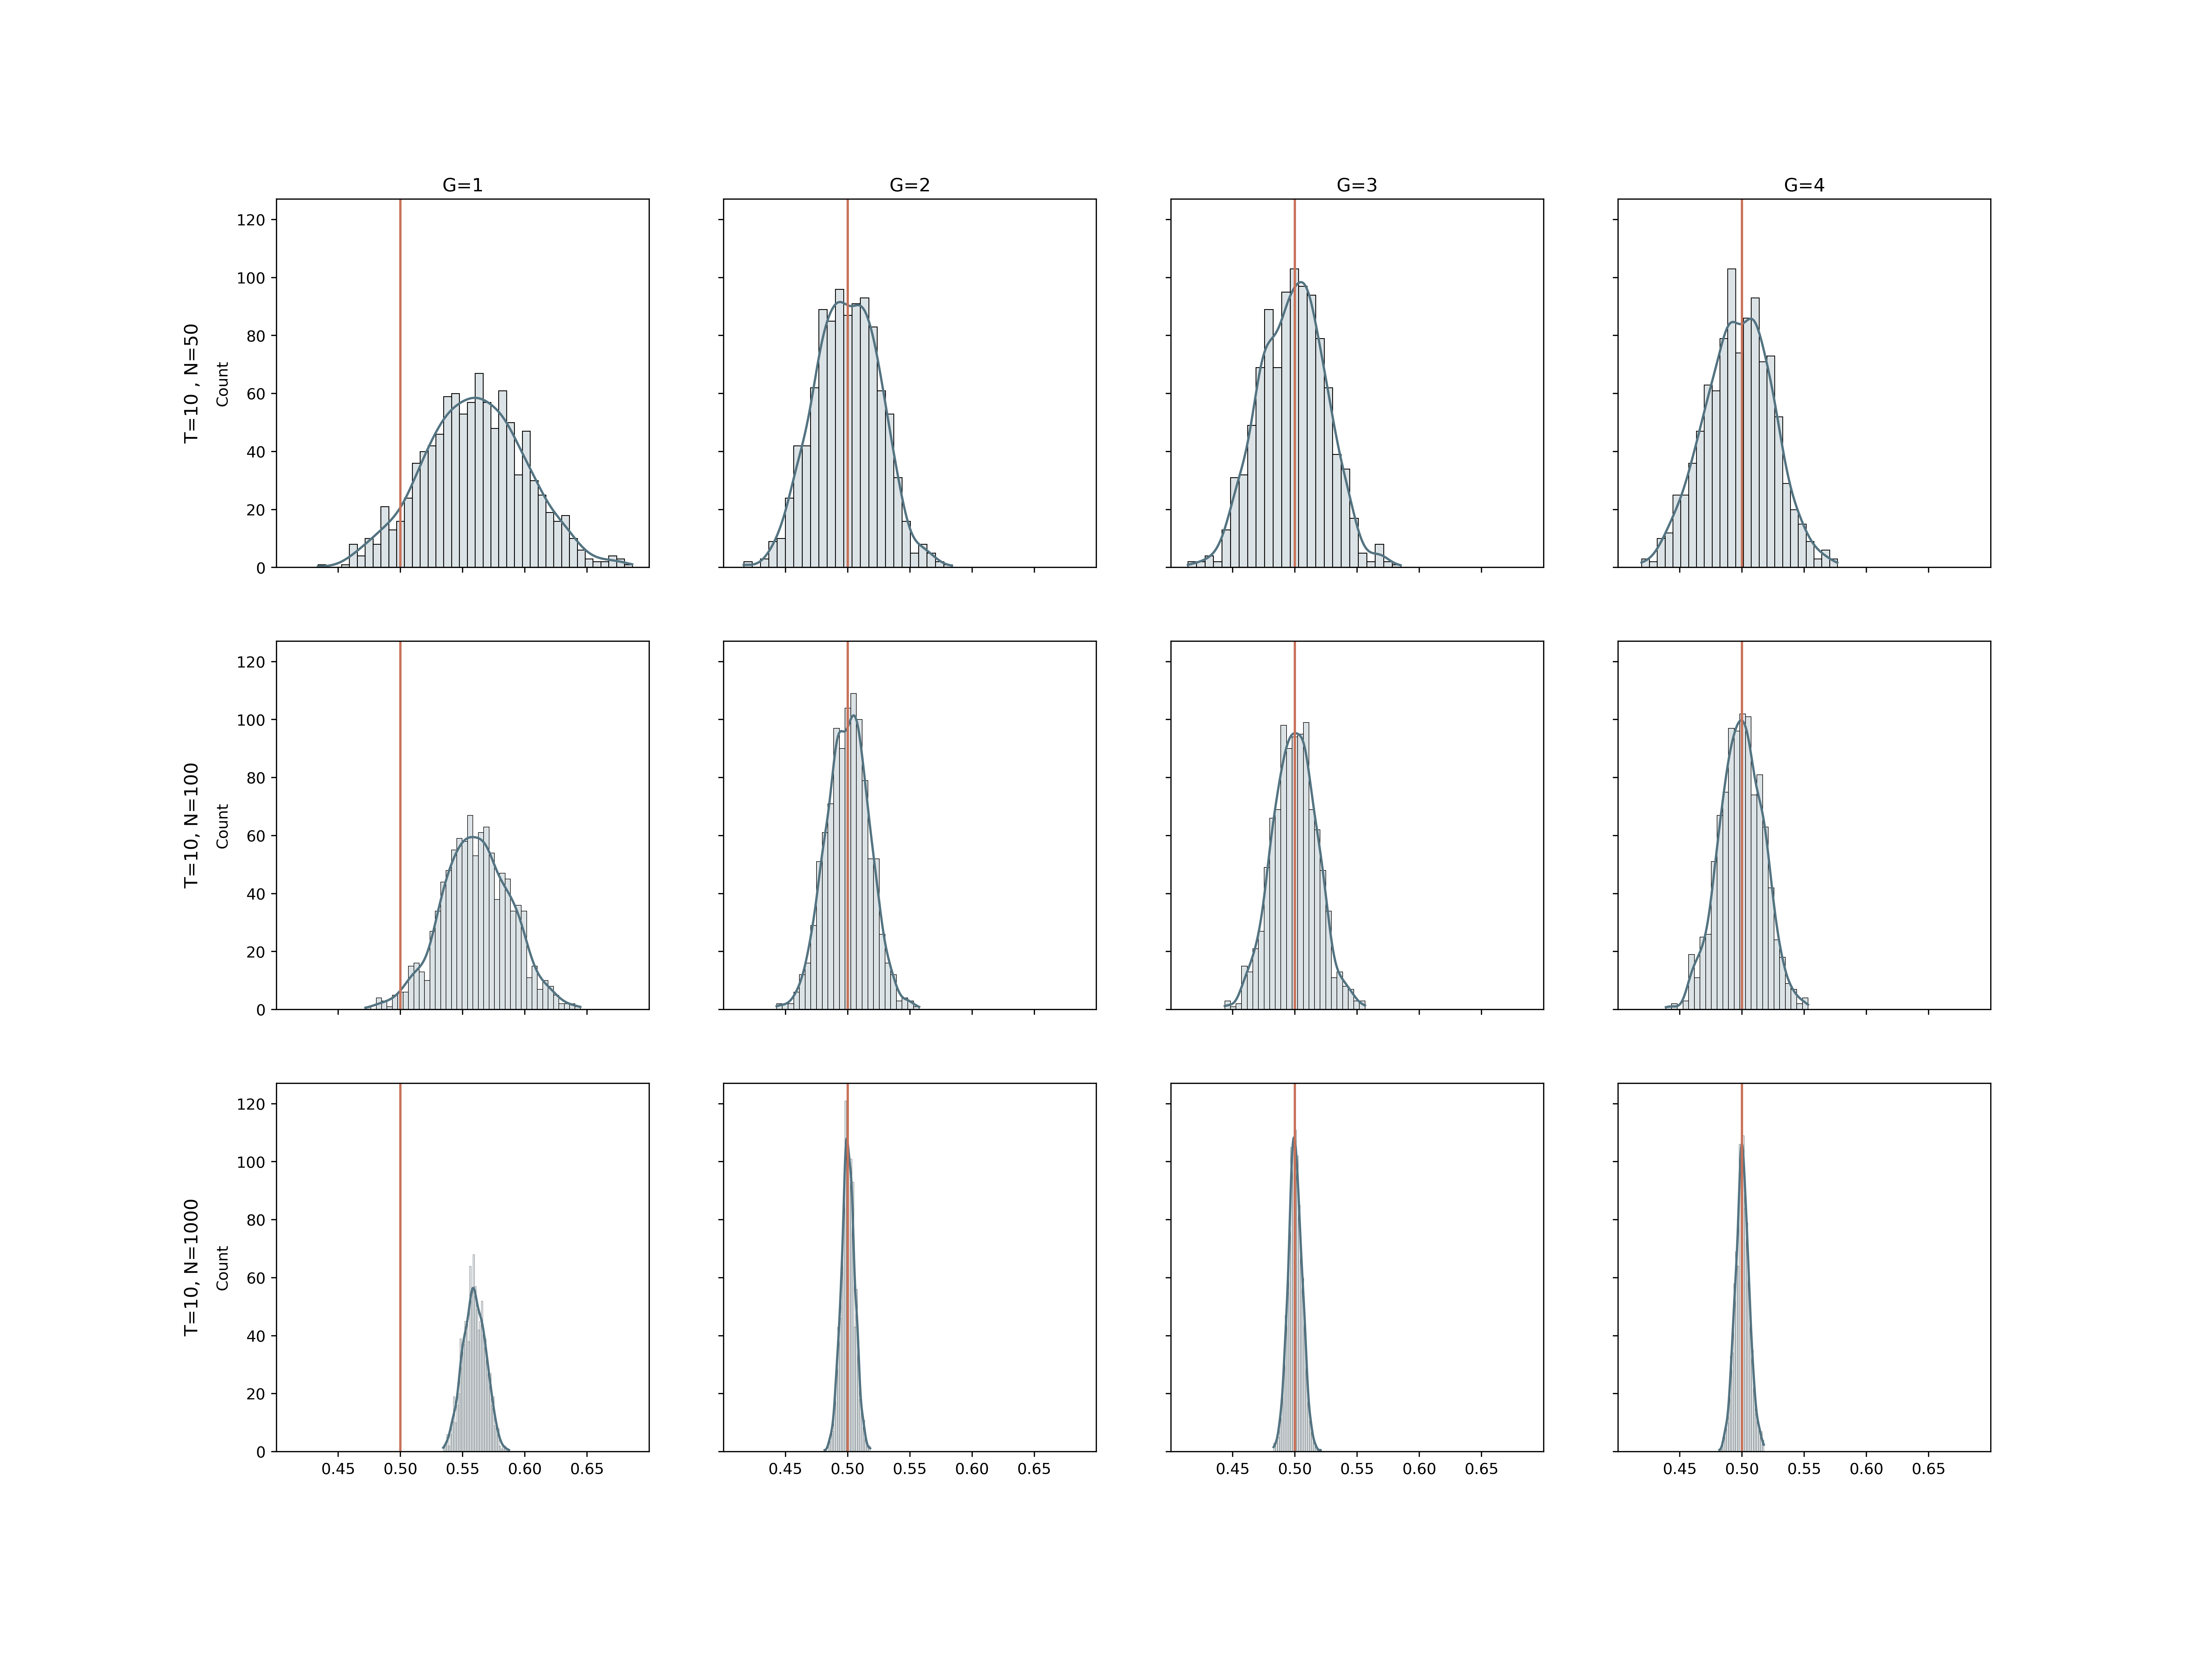
\includegraphics[scale=0.31]{sections/appendix/groupssamplingplotN.png}
\end{flushleft}
\caption{Sampling Distribution of $\hat{\theta_2}$ when T=10 and N increases in different number of group specifications where $G^0 = 2$.}
\label{fig:gsn}
\end{figure}

\begin{figure}[h]
\begin{flushleft}
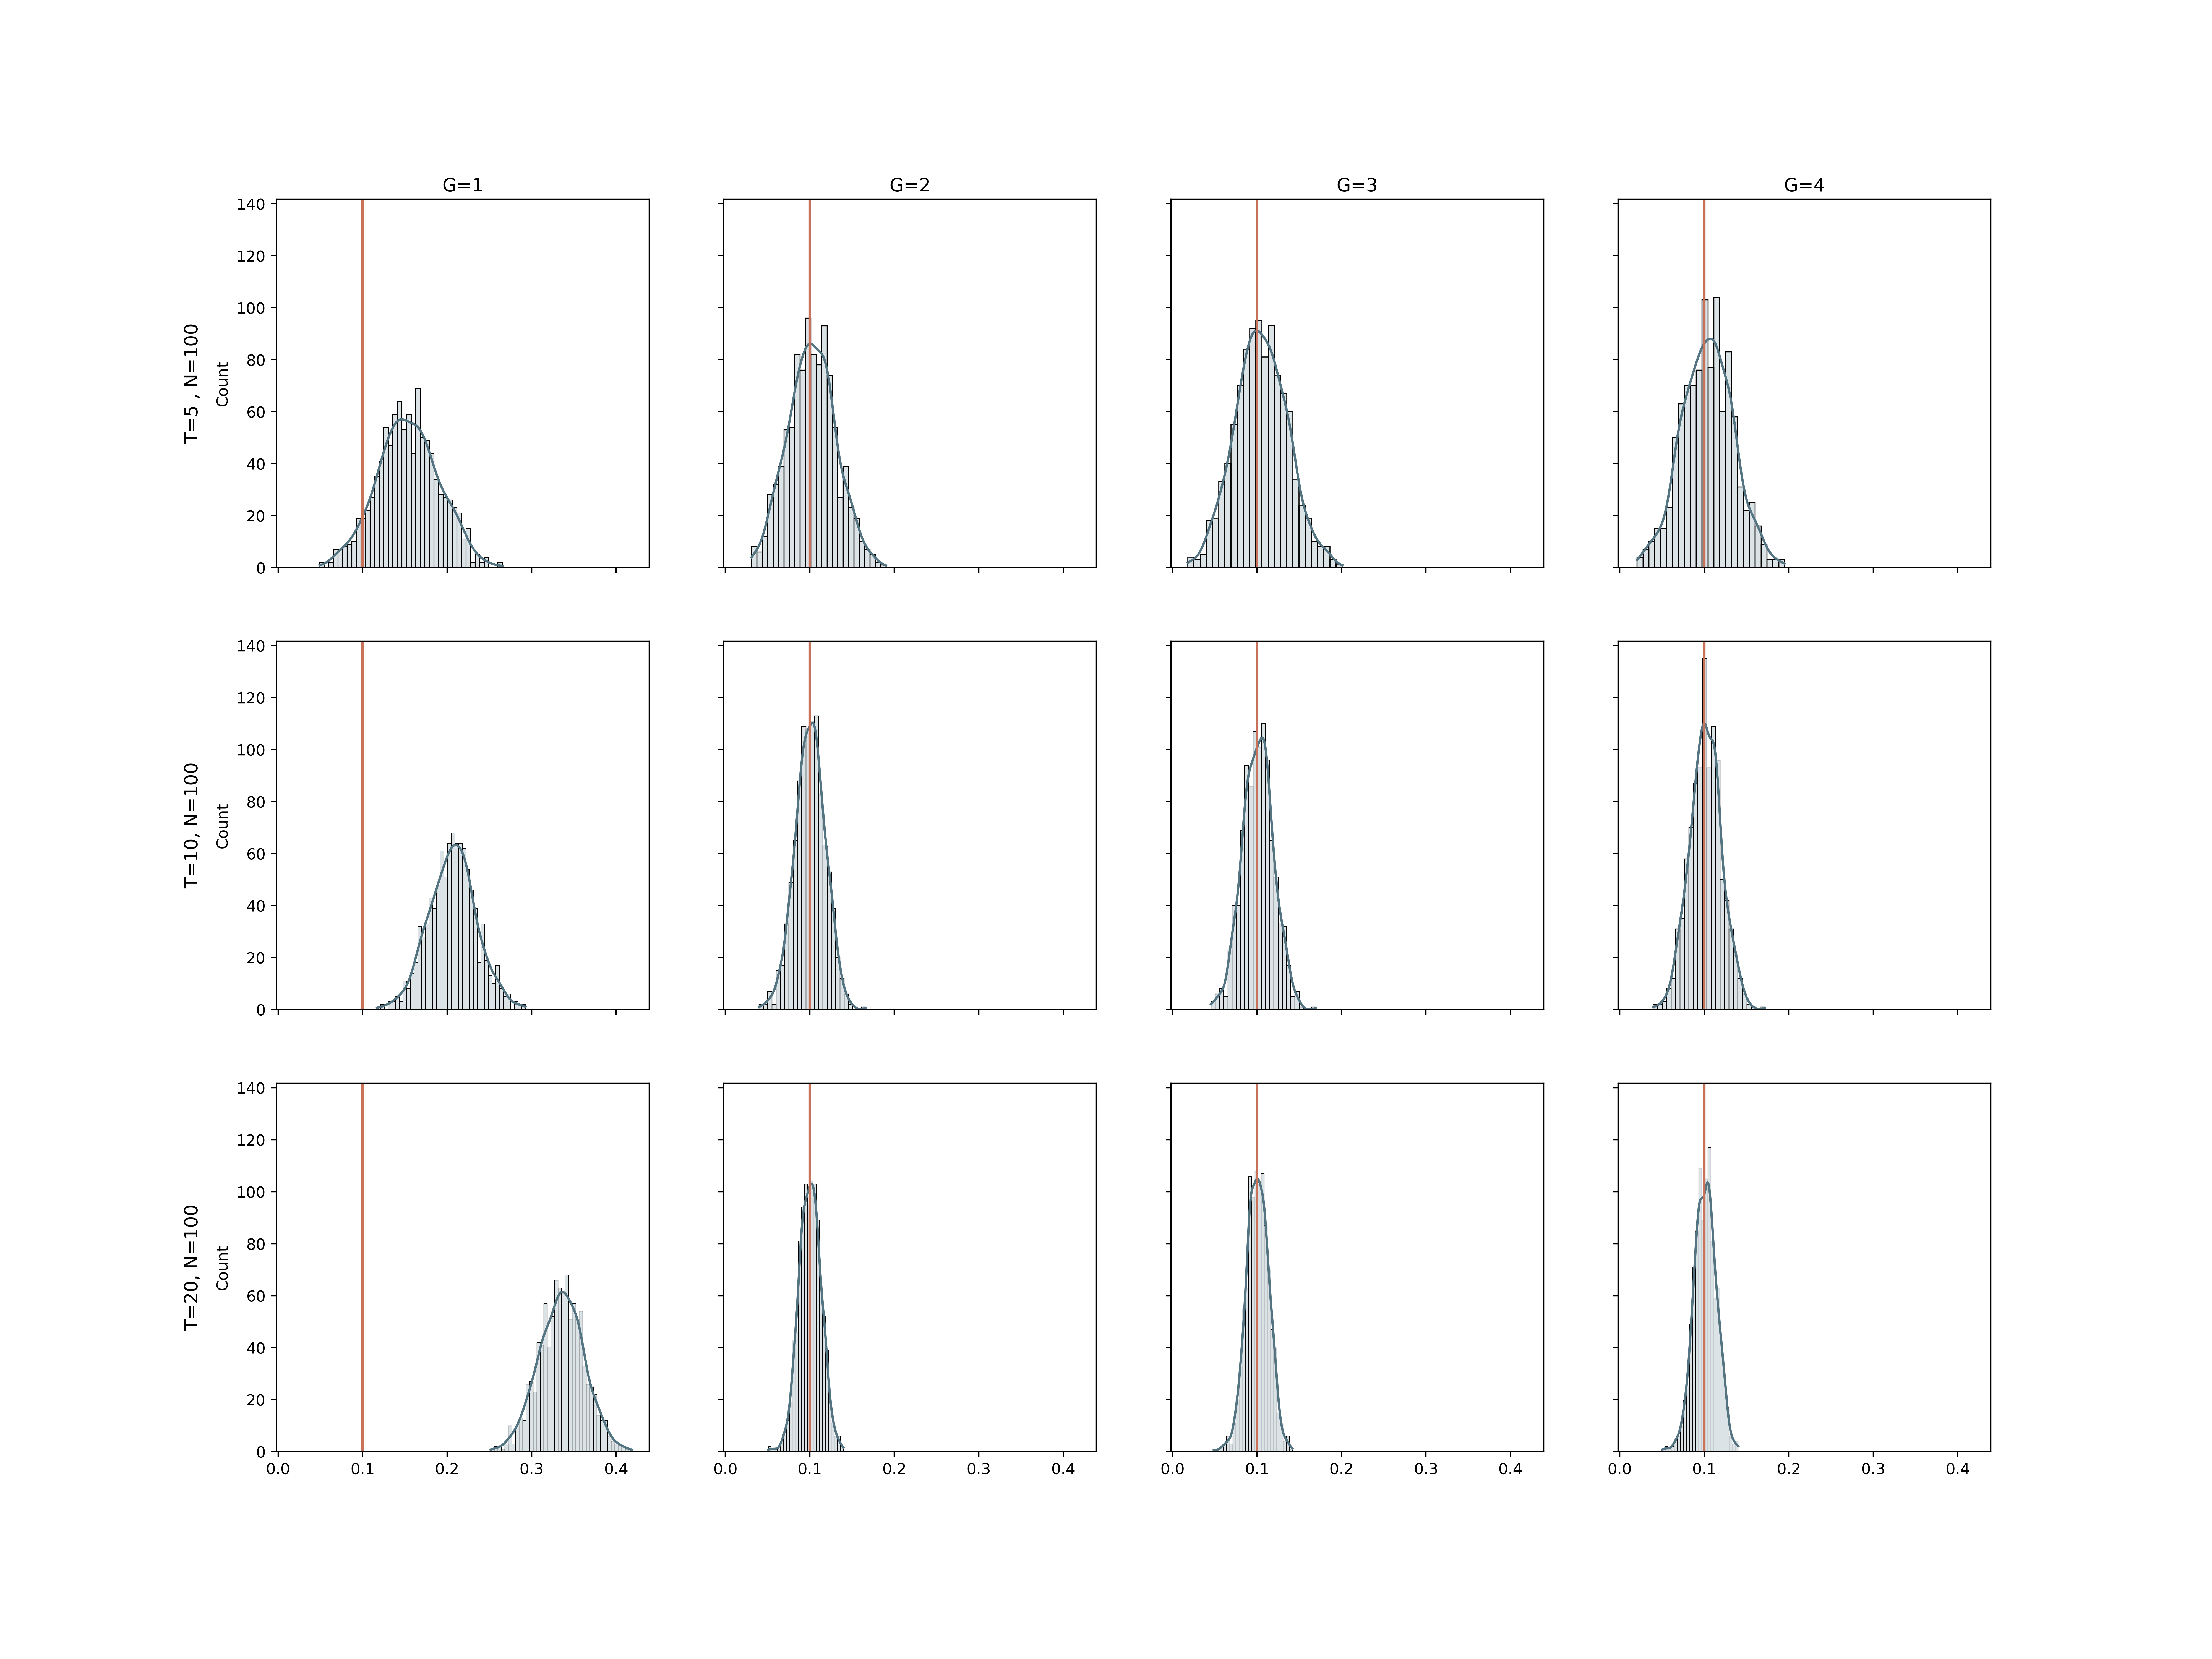
\includegraphics[scale=0.31]{sections/appendix/groupssamplingplotT1.png}
\end{flushleft}
\caption{Sampling Distribution of $\hat{\theta_1}$ when N=100 and T increases in different number of group specifications where $G^0 = 2$.}
\label{fig:gsn}
\end{figure}

\begin{figure}[h]
\begin{flushleft}
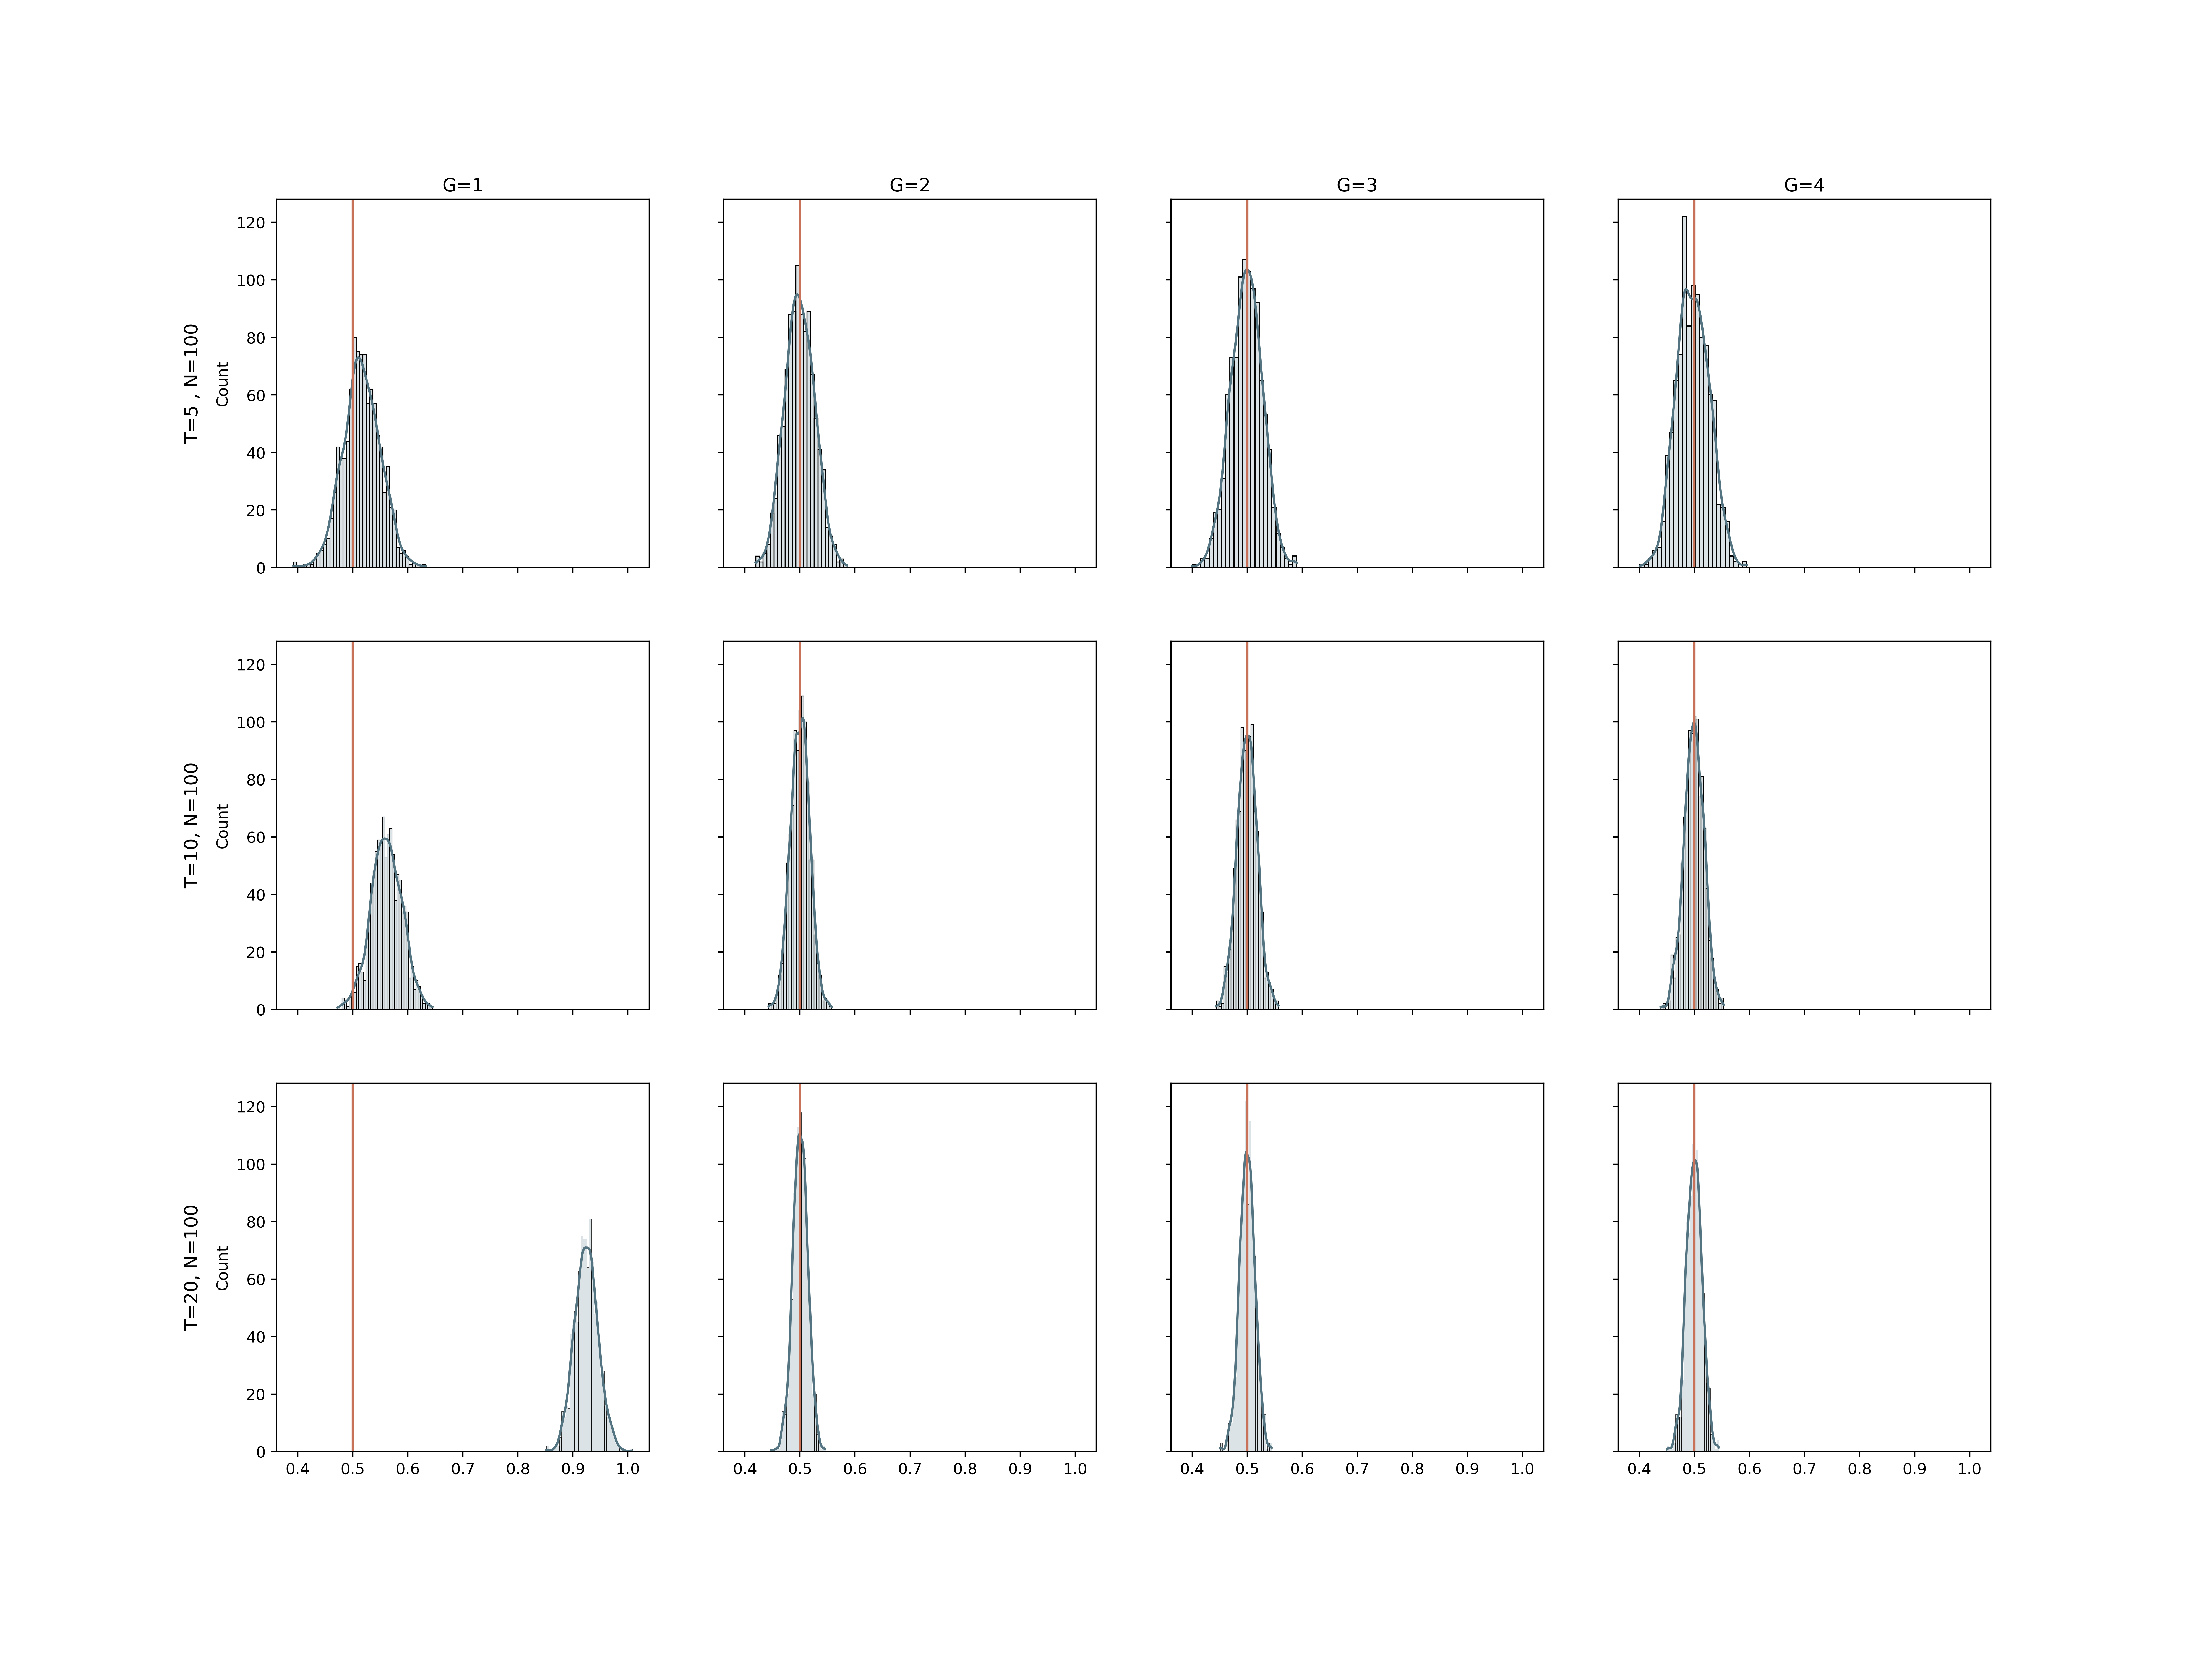
\includegraphics[scale=0.31]{sections/appendix/groupssamplingplotT.png}
\end{flushleft}
\caption{Sampling Distribution of $\hat{\theta_2}$ when N=100 and T increases in different number of group specifications where $G^0 = 2$.}
\label{fig:gsn}
\end{figure}



\begin{figure}[h]
\begin{center}
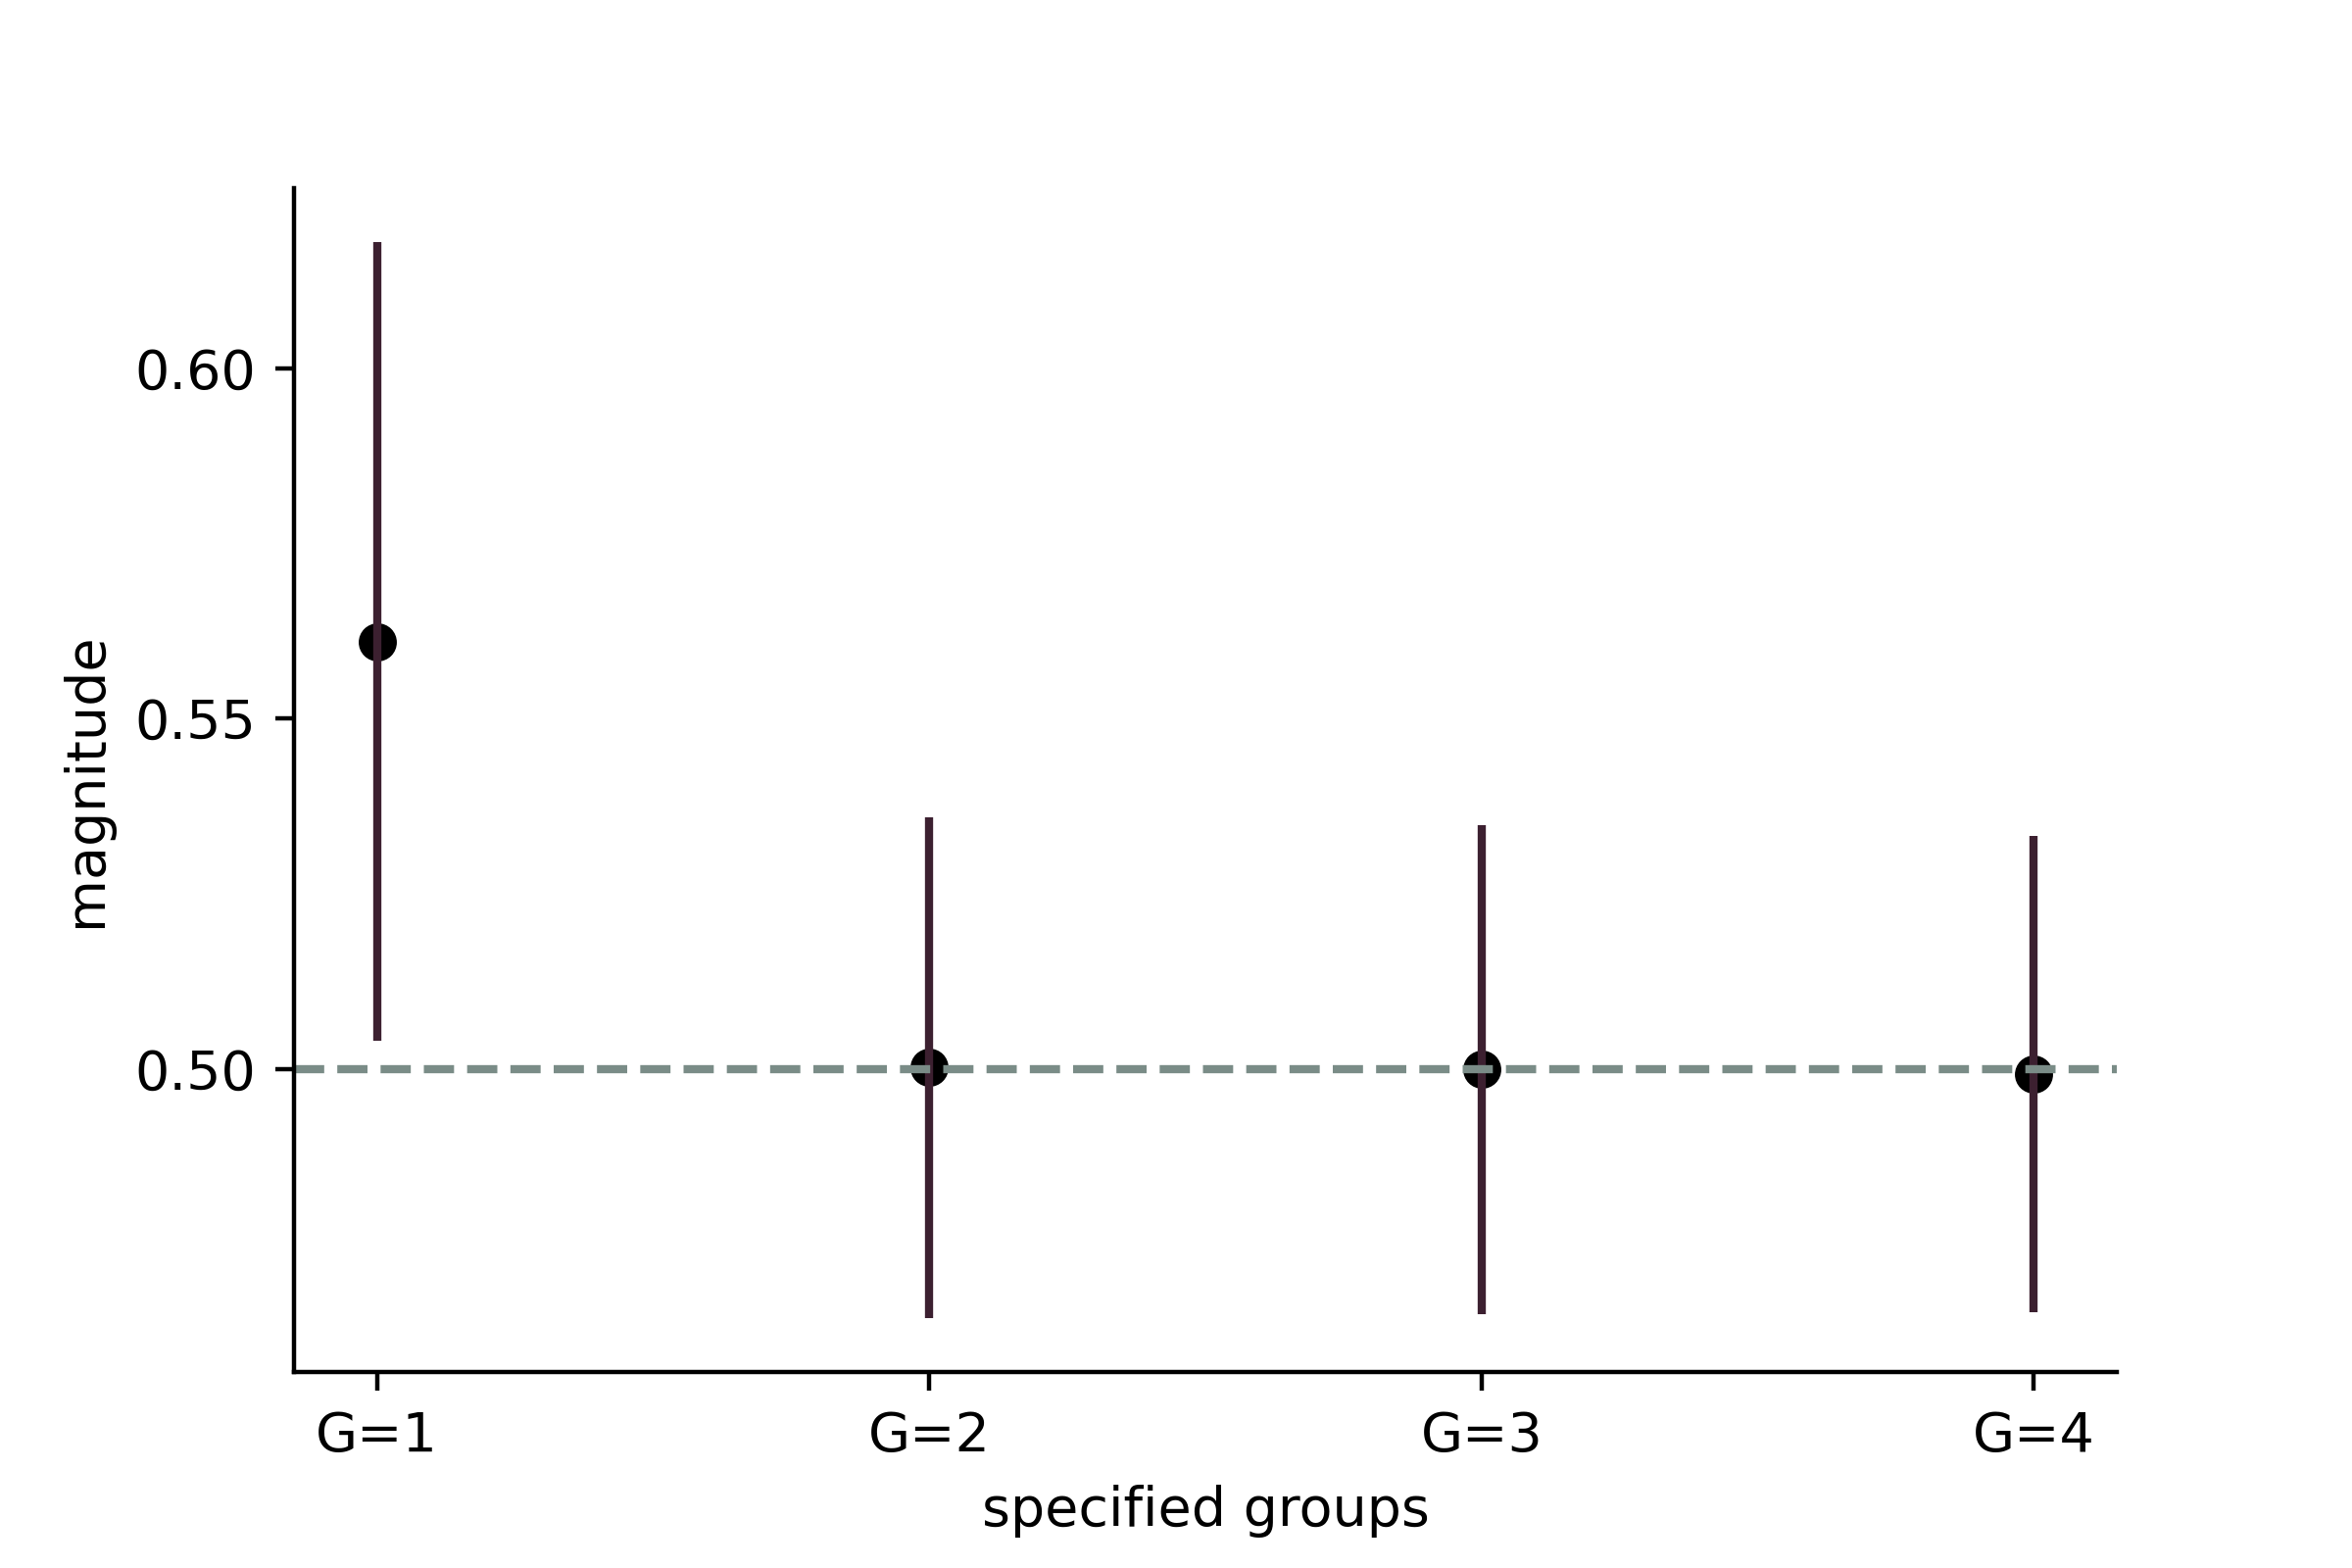
\includegraphics[scale=0.85]{sections/appendix/ciplottheta2.png}
\end{center}
\caption{Expected Value and Average Confidence Intervals of $\hat{\theta}_2$, T=10, N=100.}
\label{fig:ci2}
\end{figure}


%Proofs of WLLN and CLT are omitted.
%\subsection{Weak Law of Large Numbers}
%How to cite? My source here are chapter 4 of Michael's Econometric Basic Module WS 19/20 notes and Joachim's 5th handout of Econometrics I WS 19/20 which is from Casella and Berger (2001), Section 5.5..

Suppose $\{X_1, \dots, X_n\}$ is a sequence of i.i.d. $\mathbb{R}^k$ valued random variables  i.e. a random sample from a distribution.
Let $\Bar{X}_n$ denote the sample mean $\dfrac{1}{N}\sumi X_i$ and $\EX(X_n)$ exists then $\Bar{X}_n \overset{p}{\to} \EX(X_n)$. 

In the case where $X_i$ and $X_j$ for $i \neq j$ is not independent
but uncorrelated random variables, we would additionally need to assume existence of the variance to get this result.


\subsection{Central Limit Theorem}

Suppose $\{X_1, \dots, X_n\}$ is a sequence of i.i.d. $\mathbb{R}^k$ valued random variables and suppose $\EX(X_n) = \mu$ and $Cov(X_n)= \Sigma$ exists, then $\sqrt{n}(\Bar{X}_n - \mu) \sim \mathcal{N}(0,\Sigma)$.

\subsection{Continuous Mapping Theorem}

Suppose $\{X_1, \dots, X_n\}$ is a sequence of i.i.d. $\mathbb{R}^k$ valued random variables and g: $\mathbb{R}^k \rightarrow \mathbb{R} $ is a continuous function:
\begin{itemize}
    \item If $X_n \overset{p}{\to} X$ then  $g(X_n) \overset{p}{\to} g(X)$.
    \item If $X_n \overset{d}{\to} X$ then  $g(X_n) \overset{d}{\to} g(X)$.
\end{itemize}


%\subsection{Proof of Theorem 2.1: Consistency of Pooled OLS}

Under assumption $\mathcal{P}$, $\hat\theta_{pool}$ is identified as:
\begin{align*}
    \hat\theta_{pool} = (\sumt \sumi  x_{it}x_{it}')^{-1}\sumi\sumt x_{it}y_{it}
\end{align*}
When we plug in the model $y_{it} =  x_{it}'\theta + e_{it}$:

\begin{align*}
    \hat\theta_{pool} = (\sumt \sumi x_{it}x_{it}')^{-1}\sumt\sumi x_{it}x_{it}'\theta + (\sumt \sumi x_{it}x_{it}')^{-1} \sumt \sumi  x_{it}e_{it} \\
    = \theta + (\sumt \sumi x_{it}x_{it}')^{-1} \sumt \sumi x_{it}e_{it}\\
    = \theta + (\sumt \dfrac{1}{N} \sumi  x_{it}x_{it}')^{-1} \sumt \dfrac{1}{N} \sumi x_{it}e_{it}
\end{align*}
By assumption $\mathcal{P}$-1 and WLLN for i.i.d. random variables as N $\rightarrow \infty$:
\begin{align*}
\sumt \dfrac{1}{N} \sumi x_{it}x_{it}'  \overset{p}{\to} \EX(x_{it}x_{it}') \\
\sumt \dfrac{1}{N} \sumi x_{it}e_{it}  \overset{p}{\to} \EX(x_{it}e_{it}) 
\end{align*}

By assumption $\mathcal{P}$-2 $\EX(x_{it}e_{it}) = 0$.
Thus:
\begin{align*}
 \hat\theta_{pool} \overset{p}{\to} \theta + \EX(x_{it}x_{it}')^{-1}  \EX(x_{it}e_{it})\\
 \overset{p}{\to} \theta + \EX(x_{it}x_{it}')^{-1}0\\
 \overset{p}{\to} \theta 
\end{align*}
This shows that $\hat\theta_{pool}$ is a consistent estimator of $\theta$ when assumption $\mathcal{P}$ holds. 

%\subsection{Proof of Theorem 2.2: Asymptotic Normality of Pooled OLS}
By CLT:
\begin{align*}
    \dfrac{1}{\sqrt{N}} \sumi X_i e_i \overset{d}{\to} \mathcal{N}(0,\EX(X_i'e_ie_i'X_i)),
\end{align*}
and therefore from the property of multivariate normal distribution, that is $AZ + b \sim \mathcal{N}(b,AA')$ if $Z \sim \mathcal{N}(0,\textbf{I}_k)$, $A \in \mathbb{R}^{m\times k}$, $b \in \mathbb{R}^m$, the asymptotic normality of $\hat\theta_{pool}$ follows: 
\begin{align*}
    \sqrt{N}(\hat\theta_{pool} - \theta) \overset{d}{\to} \mathcal{N}(0,\EX(X_i'X_i)^{-1}\EX(X_i'e_ie_i'X_i)\EX(X_i'X_i)^{-1})
\end{align*}


% TO-DO:
% Writing
% - Intro, June 9
% - Add FE, June 10
% - Model overview, June 11
% - report on results, June 8



% Computing:
% 1. length of confidence intervals,(June 8)
% 2. model selection: t-test, AIC-BIC,(June 8, 9, June 10)
% 3. check the objection function with different starting values of alpha. (June 11)
% 4. Application (June 11, June 12, June 13)


% - make the table 1 readable, maybe separate into a few tables.Find a good name, round-up the numbers/multiply by 100(it should be with respect to the true values(0.1, 0.5)) maybe add stars to the ones with CP above 95\%, remove the hats from parameter, 

% - incidental parameter bias


% - Add proof of why is smaller than infinity is equal to smaller than M 

% \newpage
% \begin{table}[h!]
% \centering
% \begin{center}
%  %\scalebox{0.75}{
% \input{tables/yetanothertrial}
% %}
% \end{center}
% \caption{OLS, FE, TWFE, GFE.}
% \label{tab:new}
% \end{table}


% \newpage
% \begin{table}[h!]
% \centering
% \begin{center}
% \scalebox{0.58}{
% \input{tables/andanothertrial}
% }
% \end{center}
% \caption{OLS, FE, TWFE, GFE.}
% \label{tab:results_splines}
% \end{table}

% \newpage

% \begin{table}[h!]
% \centering
% \begin{center}
% \scalebox{0.7}{
% \input{tables/bias_groups}
% }
% \end{center}
% \caption{Bias.}
% \label{tab:bias}
% \end{table}

% \begin{table}[h!]
% \centering
% \begin{center}
% \scalebox{0.7}{
% \input{tables/rmse_groups}
% }
% \end{center}
% \caption{RMSE}
% \label{tab:rmse}
% \end{table}

% \begin{table}[h!]
% \centering
% \begin{center}
% \scalebox{0.7}{
% \input{tables/cp_groups}
% }
% \end{center}
% \caption{Coverage Probability.}
% \label{tab:cp}
% \end{table}

% Error in the code for T=20, N=50, G=3.

% \newpage
% \begin{figure}[h!]
% \centering
% \includegraphics[scale=0.33]{sens.png}
% \caption{Sampling plots with true values as starting values}
% \label{fig:hşstogram}
% \end{figure}

% \begin{figure}[h!]
% \centering
% \includegraphics[scale=0.33]{simplotsens.png}
% \caption{Sampling plots with diverted starting values}
% \label{fig:hşstogram}
% \end{figure}

